%% LyX 2.4.0~beta5 created this file.  For more info, see https://www.lyx.org/.
%% Do not edit unless you really know what you are doing.
\documentclass[english]{foils}
\usepackage[T1]{fontenc}
\usepackage{textcomp}
\usepackage[latin9]{inputenc}
\pagestyle{foilheadings}
\setcounter{secnumdepth}{1}
\setcounter{tocdepth}{1}
\usepackage{color}
\usepackage{url}
\usepackage{amsmath}
\usepackage{amsthm}
\usepackage{amssymb}
\usepackage{graphicx}

\makeatletter
%%%%%%%%%%%%%%%%%%%%%%%%%%%%%% Textclass specific LaTeX commands.
\theoremstyle{definition}
\newtheorem{defn}{\protect\definitionname}
\theoremstyle{plain}
\newtheorem{thm}{\protect\theoremname}
\newenvironment{lyxcode}
	{\par\begin{list}{}{
		\setlength{\rightmargin}{\leftmargin}
		\setlength{\listparindent}{0pt}% needed for AMS classes
		\raggedright
		\setlength{\itemsep}{0pt}
		\setlength{\parsep}{0pt}
		\normalfont\ttfamily}%
	 \item[]}
	{\end{list}}
\theoremstyle{remark}
\newtheorem{rem}{\protect\remarkname}

%%%%%%%%%%%%%%%%%%%%%%%%%%%%%% User specified LaTeX commands.
\usepackage{xcolor}
\renewcommand{\labelitemi}{$\textcolor{blue}{\bullet}$}
\renewcommand{\labelitemii}{$\textcolor{teal}{\Rightarrow}$}
\renewcommand{\labelitemiii}{$\textcolor{red}{\rightarrow}$}
\renewcommand{\labelitemiv}{$\textcolor{brown}{\circ}$}
% for French theorems, etc. since I'm using English to fix bullet pb.
\providecommand{\examplename}{Example}
\providecommand{\definitionname}{Definition}
\providecommand{\theoremnname}{Theorem}
\providecommand{\remarkname}{Remark}
\providecommand{\exercisename}{Exercise}
% DT book stuff
\newcommand{\argmin}{\operatornamewithlimits{argmin}} % for a "clean" argmin 
\newcommand{\T}{\mathrm{T}}  % transpose
\newcommand{\PP}{\mathrm{P}}  % probability
\newcommand{\dd}{\mathrm{d}} % integration dx
\newcommand{\ee}{\mathrm{e}} % exponential
\newcommand{\E}{\mathrm{E}} % expectation
%_%_%_%_%_%_%_%_
% for tikz drawings and cartoons
%_%_%_%_%_%_%_%_

\usepackage{tikz}

% for tikzit drawings
\usepackage{tikzit}
\input{flow.tikzstyles}


% for decision trees:
\tikzset{
	treenode/.style = {shape=rectangle, rounded corners,
		draw, align=center,
		top color=white, bottom color=blue!20},
	root/.style     = {treenode, font=\Large, bottom color=red!30},
	env0/.style     = {treenode, font=\large, bottom color=orange!30},
	env1/.style     = {treenode,  bottom color=green!30},
	env/.style      = {treenode, font=\ttfamily\normalsize},
    leaf/.style      = {treenode, font=\ttfamily\normalsize},
	dummy/.style    = {circle,draw}
}
\usetikzlibrary{positioning}

%_%_%_%_%_%_%_%_%_%_
% for algorithms and listings
%_%_%_%_%_%_%_%_%_%_

%\usepackage{algorithm_MA,algpseudocode}
%\usepackage{algorithmic}
\usepackage{algpseudocode}

%\floatstyle{ruled}
%\newfloat{algorithm}{tbp}
%\providecommand{\algorithmname}{Algorithm}
%\floatname{algorithm}{\protect\algorithmname}
%

% try and fix \Comment problem due to excessive defs in Chap. DA
\algrenewcommand{\algorithmiccomment}[1]{%
	\hfill$\triangleright$\ \textcolor{darkgray}{#1}}

\makeatother

\usepackage{babel}
\providecommand{\definitionname}{Definition}
\providecommand{\remarkname}{Remark}
\providecommand{\theoremname}{Theorem}

\begin{document}

\MyLogo{SciML: Lecture 02 - Optimization}
\title{SciML - Gradients and Optimization}
\author{Mark Asch - IMU/VLP/CSU }
\date{2023}
\maketitle

\foilhead{Program}
\begin{enumerate}
\item Optimization:
\begin{enumerate}
\item \textcolor{red}{Gradients and Optimization.}
\item Automatic Differentiation: Computational Graphs, Backpropagation and
Adjoints.
\item Optimization and AD with PyTorch.
\end{enumerate}
\item Physics constrained learning (PCL).
\item Physics Induced Neural Networks (PINN).
\item Operator-based learning.
\end{enumerate}

\foilhead{$\;$}

\vfill{}

\begin{center}
{\Large\textbf{\textcolor{blue}{OPTIMIZATION, GRADIENTS}}}{\Large\par}
\par\end{center}

\vfill{}


\foilhead{Recall: Optimization}
\begin{itemize}
\item \textcolor{magenta}{Optimization} is at the very heart of:
\begin{itemize}
\item Machine Learning
\item Inverse Problems (including Data Assimilation)
\item Digital Twins
\end{itemize}
\end{itemize}
\begin{defn}
In an optimization problem, we seek the minimum of a cost function,
usually an error function describing the \textcolor{magenta}{mismatch}
between model output and observations/data/measurements.
\end{defn}
The general, \textcolor{magenta}{unconstrained} optimization problem
is
\begin{equation}
\min_{\mathbf{x}\in\mathbb{R}^{n}}f(\mathbf{x}),\label{eq:pbopt_un}
\end{equation}
or find $\mathbf{x}_{*}$ that satisfies 
\begin{equation}
\mathbf{x}_{*}=\argmin_{\mathbf{x}\in\mathbb{R}^{n}}f(\mathbf{x}),\label{eq:pbopt_uc2}
\end{equation}
where $f\colon\mathcal{\mathbb{R}}^{n}\rightarrow\mathcal{\mathbb{R}}$
is a smooth function. 

\foilhead{Recall: Gradients}
\begin{itemize}
\item Recall: gradient descent moves opposite the gradient, hence in the
direction of \textcolor{magenta}{steepest descent}
\end{itemize}
\begin{center}
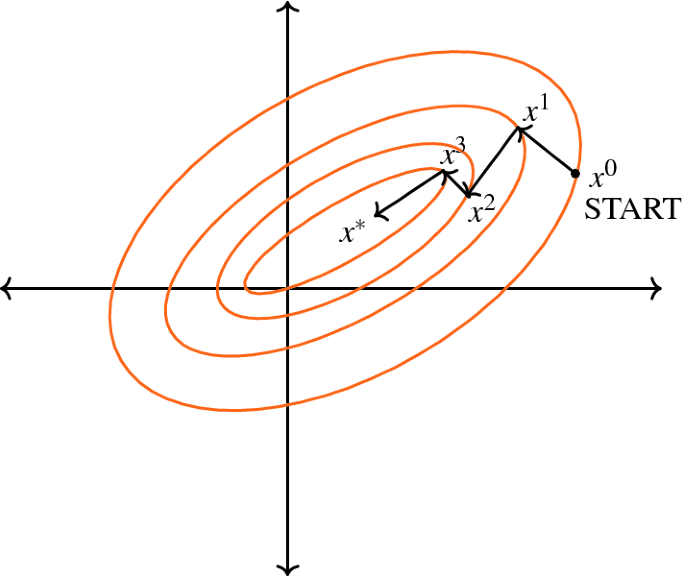
\includegraphics[scale=0.5]{graphics/sd}
\par\end{center}
\begin{itemize}
\item Necessary and sufficient conditions for finding a (local) minumum,
rely on the existence of \textcolor{magenta}{gradients} that indicate
the best direction for seeking the minimum---we just need to ``slide''
downhill \ldots{}
\end{itemize}
\begin{thm}
[Taylor's]If $f\colon\mathbb{R}^{n}\rightarrow\mathbb{R}$ is continuously
differentiable and if $\mathbf{p}\in\mathbb{R}^{n}$, then 
\[
f(\mathbf{x}+\mathbf{p})=f(\mathbf{x})+\nabla f(\mathbf{x}+t\mathbf{p})^{\T}\mathbf{p}\,,\quad t\in(0,1),
\]
where the \textcolor{magenta}{gradient vector} 
\[
\nabla f(\mathbf{x})\doteq\left(\partial f(\mathbf{x})/\partial x_{1},\ldots,\partial f(\mathbf{x})/\partial x_{n}\right)^{\T}.
\]
 Moreover, if $f\in C^{2}$ (meaning that $f$ now has two continuous
derivatives), then 
\[
\nabla f(\mathbf{x}+\mathbf{p})=\nabla f(\mathbf{x})+\int_{0}^{1}\nabla^{2}f(\mathbf{x}+t\mathbf{p})\mathbf{p}\,\dd t
\]
and 
\[
f(\mathbf{x}+\mathbf{p})=f(\mathbf{x})+\nabla f(\mathbf{x}+t\mathbf{p})^{\T}\mathbf{p}+\frac{1}{2}\mathbf{p}^{\T}\nabla^{2}f(\mathbf{x}+t\mathbf{p})\mathbf{p}
\]
for some $t\in(0,1),$ where the \textcolor{magenta}{Hessian matrix}
\[
\nabla^{2}f(\mathbf{x})\doteq\left[\begin{array}{ccc}
\dfrac{\partial^{2}f(\mathbf{x})}{\partial x_{1}^{2}} & \cdots & \dfrac{\partial^{2}f(\mathbf{x})}{\partial x_{1}\partial x_{n}}\\
\vdots & \ddots & \vdots\\
\dfrac{\partial^{2}f(\mathbf{x})}{\partial x_{n}\partial x_{1}} & \cdots & \dfrac{\partial^{2}f(\mathbf{x})}{\partial x_{n}^{2}}
\end{array}\right].
\]
\end{thm}
\begin{itemize}
\item We can now state the \textcolor{magenta}{necessary condition} for
the existence of a minimum.
\end{itemize}
\begin{thm}
[First-Order Necessary Condition]If $\mathbf{x}_{*}$ is a local
minimizer of $f,$ and if $f$ is differentiable in a neighborhood
of the point $\mathbf{x}_{*},$ then 
\begin{equation}
\nabla f(\mathbf{x}_{*})=0.\label{eq:nec_cond}
\end{equation}
\end{thm}
\begin{itemize}
\item Please see {[}1{]} for ALL the details.
\item But, as said above, the disappearance of the gradient is unfortunately
not sufficient to guarantee that $\mathbf{x}_{*}$ is a minimizer.
\begin{itemize}
\item It only implies that $f$ is \textcolor{magenta}{stationary} at $\mathbf{x}_{*}$
to first order, meaning that $f$ is insensitive to small changes,
or perturbations of $\mathbf{x}_{*}.$ 
\item But we can (and do) use this necessary condition to solve the system
of $n$ algebraic equations in $n$ unknowns defined by (\ref{eq:nec_cond}). 
\item Then we have to sort out and decide which of the candidate points
are indeed \textcolor{magenta}{minimizers}. 
\item This requires second-order information that can be obtained from the
\textcolor{magenta}{Hessian}, if and when it is available. If this
is the case, then we can state a sufficient condition for $\mathbf{x}_{*}$
to be a local minimizer.
\end{itemize}
\end{itemize}
\begin{thm}
[Second-Order Sufficient Condition] Suppose for a point $\mathbf{x}_{*}$
the function $f$ has first- and second-order derivatives. Suppose
also that the gradient of $f$ is zero and that the Hessian is positive
definite at $\mathbf{x}_{*}.$ Then $\mathbf{x}_{*}$ is a (strict)
local minimum of $f.$ 
\end{thm}
\begin{itemize}
\item The only thing that is left is an eventual condition for a \textcolor{magenta}{global
minimizer.} Apart from the definition given above, there is only one
case in which we can be sure that a local minimizer is indeed global. 
\end{itemize}
\begin{thm}
[Global Minimizer] If $f$ is a convex function, then any local minimizer
$\mathbf{x}_{*}$ of $f$ is a global minimizer. Moreover, if $f$
is differentiable, then any stationary point $\mathbf{x}_{*}$ of
$f$ is a global minimizer. 
\end{thm}

\foilhead{(Continuous, Unconstrained) Optimization Tree}
\begin{center}
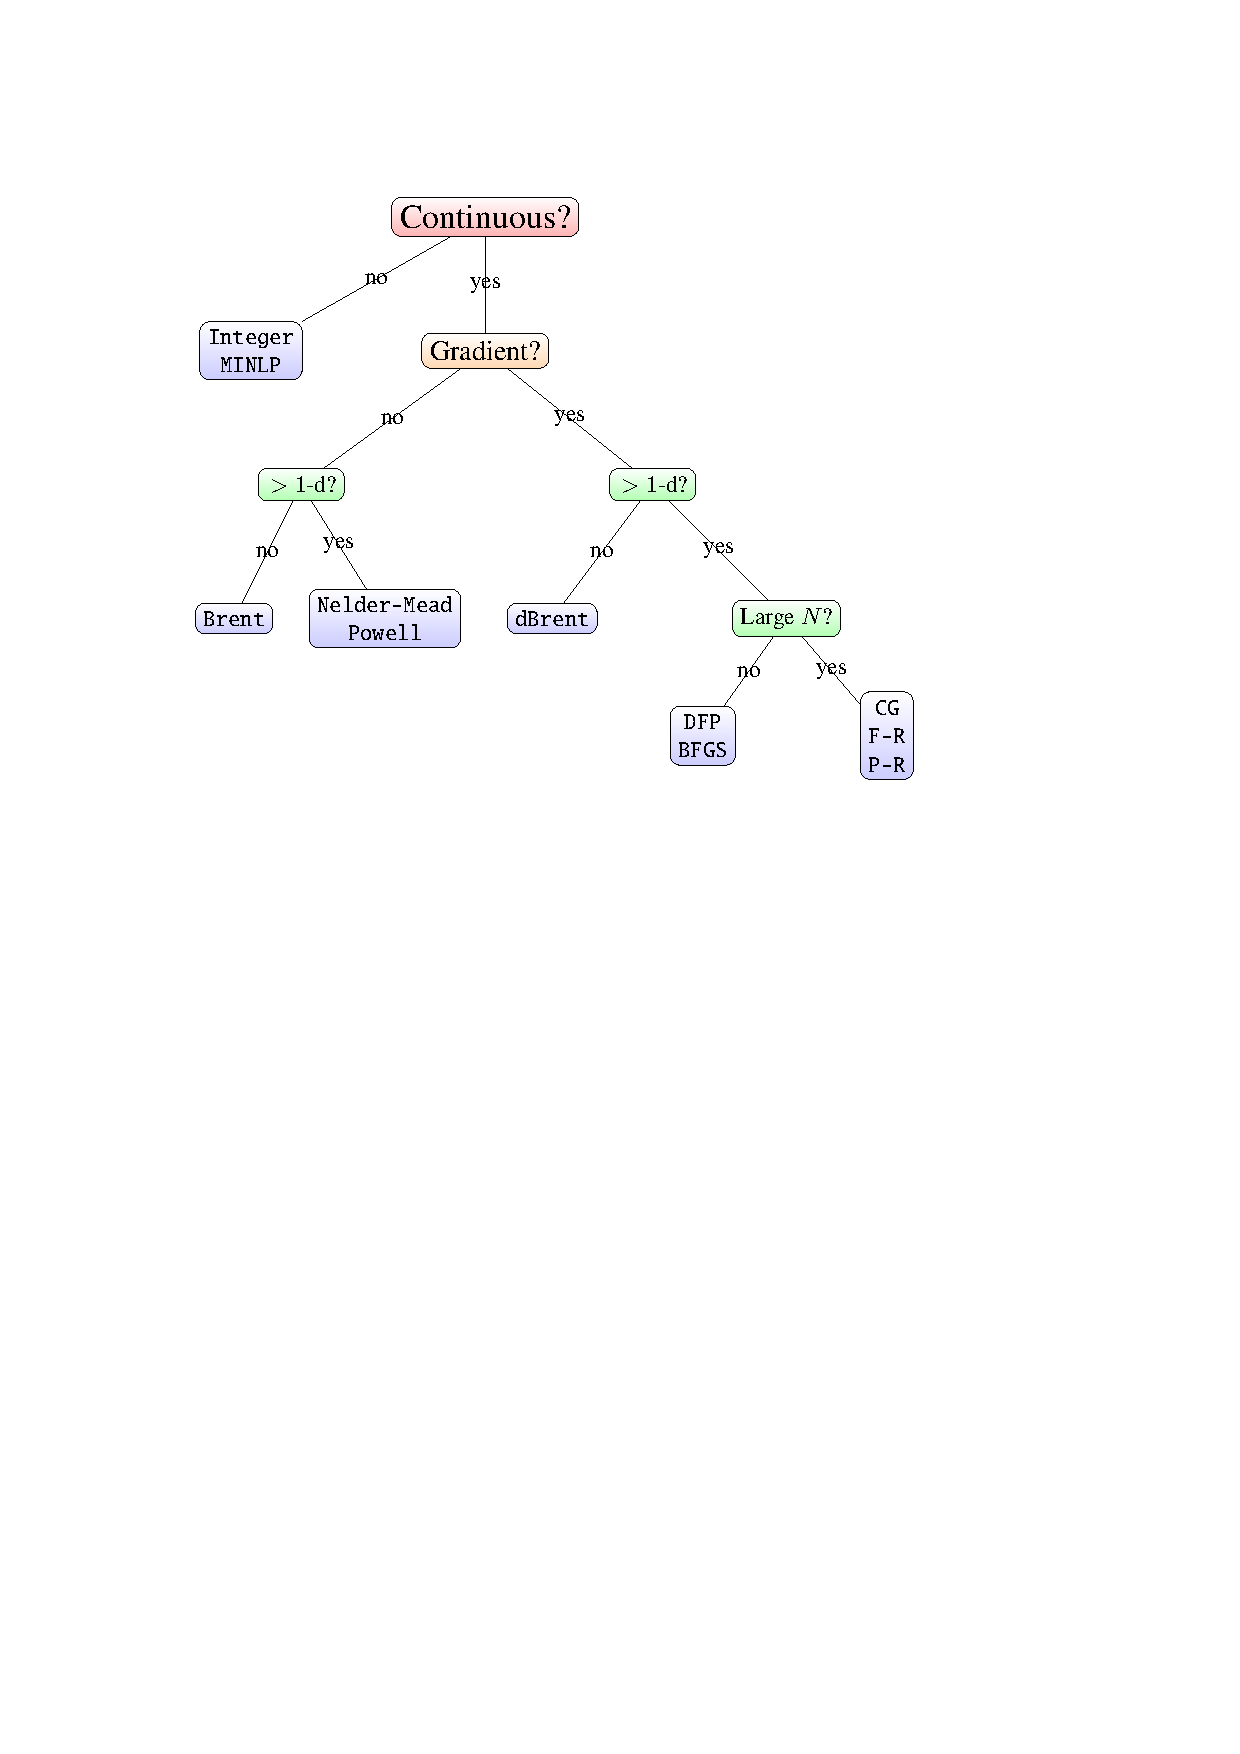
\includegraphics[width=0.8\paperwidth]{graphics/opt_tree}
\par\end{center}

Credit: \cite{Asch2022}.

\foilhead{Practical Optimization for SciML}
\begin{itemize}
\item SciML problems will usually fall into the category \textcolor{magenta}{``Large
$N$''}, since 
\begin{itemize}
\item the ML part usually implies a large number of weights
\item the inversion/assimilation process, implies a large number of iterations
\end{itemize}
\item Lower-order methods, based on \textcolor{magenta}{gradient descent}
(which is NEVER used in classical CSE) are used here:
\begin{itemize}
\item SGD (\textcolor{magenta}{stochastic gradient} descent) and its variants,
notably ADAM
\item \textcolor{magenta}{LBFGS} (quasi-Newton) when higher order is needed
and feasible
\end{itemize}
\end{itemize}

\foilhead{$\;$}

\vfill{}

\begin{center}
{\Large\textbf{\textcolor{blue}{OPTIMIZATION ALGORITHMS}}}{\Large\par}
\par\end{center}

\vfill{}


\foilhead{Recall: Gradient Descent}
\begin{itemize}
\item Recall: gradient descent moves opposite the gradient, hence in the
direction of \textcolor{magenta}{steepest descent}
\end{itemize}
\begin{center}
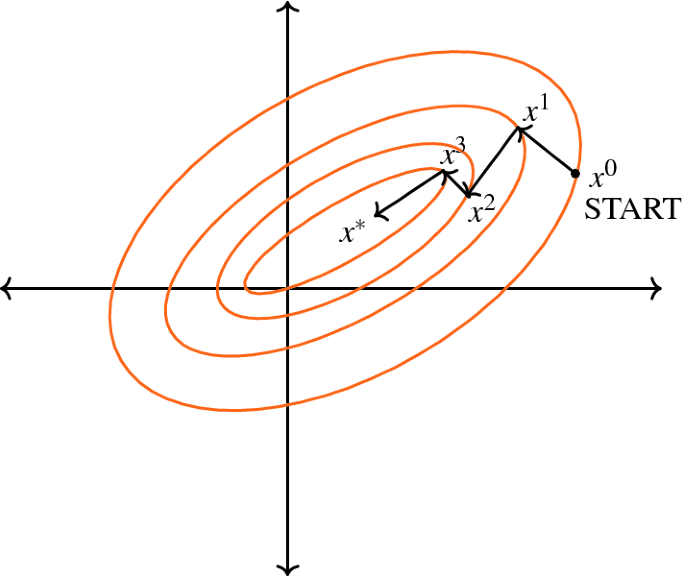
\includegraphics[scale=0.5]{graphics/sd}
\par\end{center}

\foilhead{Optimization/Minimization Algorithms}
\begin{itemize}
\item Most \textcolor{magenta}{minimization algorithms} have the following
basic structure:
\end{itemize}
\begin{lyxcode}
while~$\mathbf{x}^{(k)}$~is~not~a~minimum~~\\
~~~~calculate~the~step~direction~$\mathbf{p}^{(k)}$~

~~~~~~~~~with~$\left\Vert \mathbf{p}^{(k)}\right\Vert =1$~~\\
~~~~calculate~the~step~size~$\alpha^{(k)}$~~\\
~~~~update~$\mathbf{x}^{(k+1)}=\mathbf{x}^{(k)}+\alpha^{(k)}\mathbf{p}^{(k)}$~~\\
~~~~$k=k+1$~\\
~end.
\end{lyxcode}
\begin{itemize}
\item Gradient-based methods will use the \textcolor{magenta}{slope}, or
gradient of the function as the choice for the direction, and then
attempt to descend this slope to a lower-valued point.
\item Steepest descent uses the fact that any (differentiable) function
$f$ decreases most rapidly in the direction of $-\nabla f,$ at least
locally.
\item Then we need to solve a 1D minimization problem to find the \textcolor{magenta}{optimal
step }size (to prevent \textcolor{magenta}{overshooting}). 
\item \textbf{Steepest Gradient Descent Algorithm:}
\end{itemize}
If $f\colon\mathbb{R}^{n}\rightarrow\mathbb{R}$ is a differentiable
function and $\mathbf{x}_{0}\in\mathbb{R}^{n}$ is an initial guess,
then the following SDG algorithm computes $\mathbf{x}_{*}=\argmin_{\mathbf{x}}f(\mathbf{x}).$ 

\begin{algorithmic}[1]

\State $k=0,$ initial guess $\mathbf{x}_{0}$ \Comment{Initialization} 

\While{not converged} \Comment{Convergence criteria} 

\State $\mathbf{p}_{k}=-\nabla f(\mathbf{x}_{k})$ \Comment{Steepest
descent direction} 

\State Compute $\alpha_{k}$ that minimizes $f(\mathbf{x}_{k}+\alpha_{k}\mathbf{p}_{k})$ 

\State $\mathbf{x}_{k+1}=\mathbf{x}_{k}+\alpha_{k}\mathbf{p}_{k}$
\Comment{Update solution} 

\State $k=k+1$ \EndWhile 

\State $\mathbf{x}_{*}=\mathbf{x}_{k}$ \Comment{Output the converged
solution} 

\end{algorithmic}

\foilhead{Newton and Quasi-Newton Methods}
\begin{itemize}
\item If we have access to the \textcolor{magenta}{Hessian}, in addition
to the gradient, then we can formulate an extremely rapidly converging
algorithm, Newton's method. 
\begin{itemize}
\item However, this method is rarely used in practise-{}-{}-see explanations
below-{}-{}-and is replaced by \textcolor{magenta}{quasi-Newton} methods
that use some type of approximation of the Hessian. 
\end{itemize}
\item Newton's method supplies a local \textcolor{magenta}{quadratic approximation}
to an objective function, which is good because we can readily compute
the minimum of a quadratic function. 
\item Take a truncated Taylor series expansion of the function $f$ and
expand in the neighborhood of a point $\mathbf{x}$ up to order two.
\begin{itemize}
\item Suppose that 
\[
f\colon\mathbb{R}^{n}\rightarrow\mathbb{R}
\]
and that $f$ has two continuous derivatives. Then we can expand 
\[
f(\mathbf{x}_{k}+\mathbf{p})\approx f_{k}+\mathbf{p}^{\T}\nabla f_{k}+\frac{1}{2}\mathbf{p}^{\T}\nabla^{2}f_{k}\mathbf{p}\doteq m_{k}(\mathbf{p}),
\]
where $f_{k}=f(\mathbf{x}_{k}),$ $\nabla f$ is the\textcolor{magenta}{{}
gradient} of $f$ with $i$-th element $g_{i}=\frac{\partial f}{\partial x_{i}}$
and $\nabla^{2}f$ is its \textcolor{magenta}{Hessian}, whose $ij$-th
element is $H_{ij}=\frac{\partial^{2}f}{\partial x_{i}\partial x_{j}}$ 
\item To minimize $m_{k}$ with respect to $\mathbf{p},$ we take its gradient
and impose the\textcolor{magenta}{{} necessary condition}, $\nabla_{\mathbf{p}}m_{k}(\mathbf{p})=0,$
to obtain 
\[
0+\nabla f_{k}+\nabla^{2}f_{k}\mathbf{p}=0,
\]
from which we deduce the \textcolor{magenta}{Newton direction }
\[
\mathbf{p}^{\mathrm{N}}=-\left(\nabla^{2}f_{k}\right)^{-1}\nabla f_{k}.
\]
\item The iteration step becomes 
\[
\mathbf{x}_{k+1}=\mathbf{x}_{k}-H^{-1}(\mathbf{x}_{k})g(\mathbf{x}_{k}).
\]
\end{itemize}
\item The method is summarized in this very simple \textcolor{magenta}{Newton
algorithm}:
\end{itemize}
\begin{lyxcode}
$\mathbf{x}=\mathbf{x}_{0}$~~\\
~\textbf{for~$k=0,1,2,...$}~~\\
~~~~solve~$\nabla^{2}f(\mathbf{x}_{k})\mathbf{p}_{k}=-\nabla f(\mathbf{x}_{k})$~~\\
~~~~$\mathbf{x}_{k+1}=\mathbf{x}_{k}+\mathbf{p}_{k}$~~\\
~\textbf{end}
\end{lyxcode}
\begin{itemize}
\item The convergence is local, but \textcolor{magenta}{quadratic}, which
is extremely rapid. However, Newton's method has\textcolor{magenta}{{}
three major inconveniences}. The method can be:
\end{itemize}
\begin{enumerate}
\item \textcolor{magenta}{Unreliable} due to the (very) local convergence
and the high sensitivity to the initial guess. 
\item \textcolor{magenta}{Expensive} due to the denseness of the Hessian
matrix, especially for large $n.$ 
\item \textcolor{magenta}{Complicated} since the Hessian is invariably difficult
to compute. 
\end{enumerate}

\foilhead{Quasi-Newton: BFGS and L-BFGS}
\begin{itemize}
\item Quasi-Newton methods have been developed to overcome some of the \textcolor{magenta}{shortcomings}
of Newton's method, while still trying to use some kind of \textcolor{magenta}{second-order}
information. 
\begin{itemize}
\item The advantage will be a gain in convergence rate. 
\end{itemize}
\item These methods all use a \textcolor{magenta}{Newton-like update} of
the form 
\[
\mathbf{x}_{k+1}=\mathbf{x}_{k}-\alpha_{k}B_{k}^{-1}\nabla f(\mathbf{x}_{k}),
\]
where
\begin{itemize}
\item $\alpha_{k}>0$ is the usual \textcolor{magenta}{linesearch} parameter 
\item $B_{k}$ is some \textcolor{magenta}{approximation to the Hessian}
matrix. 
\end{itemize}
\item This can be written, in general, as 
\[
\mathbf{x}_{k+1}=\mathbf{x}_{k}+\mathbf{d}_{k},
\]
where 
\begin{equation}
\mathbf{d}_{k}=-\alpha_{k}B_{k}^{-1}\nabla f(\mathbf{x}_{k})\label{eq:dk}
\end{equation}
is the descent direction. 
\item Note that:
\begin{itemize}
\item When $B_{k}=I,$ we have the \textcolor{magenta}{gradient descent
}method, and when $\alpha_{k}=1,$ steepest decent. 
\item When $B_{k}=\nabla^{2}f(\mathbf{x}_{k}),$ $\alpha_{k}=1,$ we have
\textcolor{magenta}{Newton's} method. 
\item When $B_{k}$ is an approximation of the Hessian, we obtain a \textcolor{magenta}{quasi-Newton}
method. 
\end{itemize}
\item We now consider the construction of appropriate\textcolor{magenta}{{}
approximation }expressions for $B_{k}.$ There are two commonly used
formulations, 
\begin{itemize}
\item the Broyden-Fletcher-Goldfarb-Shanno (\textcolor{magenta}{BFGS})\index{optimization!quasi Newton methods!BFGS}
and 
\item the Davidon-Fletcher-Powell (DFP)\index{optimization!quasi Newton methods!DFP}
methods. 
\end{itemize}
\item Both are what are called \textcolor{magenta}{low-rank updates}, 
\[
B_{k+1}=B_{k}+B_{k}^{\mathrm{u}}\,,
\]
that iteratively build up an approximation $B_{k}$ of the Hessian,
starting (usually) from the initial guess $B_{0}=I,$ the steepest
gradient descent direction, and using an update matrix of the form
\[
B_{k}^{\mathrm{u}}=a\mathbf{u}\mathbf{u}^{\T}+b\mathbf{v}\mathbf{v}^{\T},
\]
where $a$ and $b$ are scalars, and $\mathbf{u}$ and $\mathbf{v}$
are vectors that satisfy a secant condition.
\item It can then be rigorously proven that the resulting $B_{k}$ is indeed
a good, symmetric, positive-definite matrix that ensures that $\mathbf{d}_{k}$
is a descent direction. 
\item The \textcolor{magenta}{BFGS update }is given by
\end{itemize}
\begin{equation}
B_{k+1}=B_{k}-\frac{B_{k}\mathbf{s}_{k}\mathbf{s}_{k}^{\T}B_{k}}{\mathbf{s}_{k}^{\T}B_{k}\mathbf{s}_{k}}+\frac{\mathbf{y}_{k}\mathbf{y}_{k}^{\T}}{\mathbf{y}_{k}^{T}\mathbf{s}_{k}},\label{eq:BFGS}
\end{equation}

where we have defined 
\[
\mathbf{s}_{k}=\mathbf{x}_{k+1}-\mathbf{x}_{k},\qquad\mathbf{y}_{k}=\nabla f_{k+1}-\nabla f_{k}.
\]

\begin{itemize}
\item The \textcolor{magenta}{DFP update} is given by 
\begin{equation}
B_{k+1}=(I-\gamma_{k}\mathbf{y}_{k}\mathbf{s}_{k}^{\T})B_{k}(I-\gamma_{k}\mathbf{s}_{k}\mathbf{y}_{k}^{\T})+\gamma_{k}\mathbf{y}_{k}\mathbf{y}_{k}^{\T},\label{eq:DFP}
\end{equation}
where 
\[
\gamma_{k}=\frac{1}{\mathbf{y}_{k}^{\T}\mathbf{s}_{k}}.
\]
\item For the implementations, it is better to use directly the inverse,
\[
H_{k}=B_{k}^{-1},
\]
since it enables a direct computation of the search direction with
a simple matrix-vector multiplication. 
\begin{itemize}
\item The \textcolor{magenta}{Sherman-Morrison-Woodbury} formula gives 
\begin{equation}
H_{k+1}^{\mathrm{BFGS}}=(I-\gamma_{k}\mathbf{s}_{k}\mathbf{y}_{k}^{\T})H_{k}(I-\gamma_{k}\mathbf{y}_{k}\mathbf{s}_{k}^{\T})+\gamma_{k}\mathbf{s}_{k}\mathbf{s}_{k}^{\T},\label{eq:BFGS2}
\end{equation}
and 
\begin{equation}
H_{k+1}^{\mathrm{DFP}}=H_{k}-\frac{H_{k}\mathbf{y}_{k}\mathbf{y}_{k}^{\T}H_{k}}{\mathbf{y}_{k}^{\T}H_{k}\mathbf{y}_{k}}+\frac{\mathbf{s}_{k}\mathbf{s}_{k}^{\T}}{\mathbf{y}_{k}^{\T}\mathbf{s}_{k}},\label{eq:DFP2}
\end{equation}
for the BFGS and DFP methods respectively.
\end{itemize}
\item \textbf{Algorithm:} BFGS and DFP Quasi-Newton with Linesearch
\end{itemize}
If $f\colon\mathbb{R}^{n}\rightarrow\mathbb{R}$ is a differentiable
function and $\mathbf{x}_{0}\in\mathbb{R}^{n}$ is an initial guess,
then the following Quasi-Newton algorithm computes $\mathbf{x}_{*}=\argmin_{\mathbf{x}}f(\mathbf{x}).$

\begin{algorithmic}[1] 

\State $k=0,$ initial guess $\mathbf{x}_{0}$, $f_{0}=f(\mathbf{x}_{0})$
, $\nabla f_{0}=\nabla f(\mathbf{x}_{0}),$ $H_{0}=I$ \Comment{Initialize} 

\State $\mathbf{p}_{0}=-H_{0}\nabla f_{0}$ \Comment{Initial direction
is steepest descent}

\While{not converged} \Comment{Convergence criteria} %\For{ $k = 0,1,\ldots$} \Comment{Iteration loop}
 

\State{\footnotesize{} Compute $\alpha_{k}$ to minimize $f(\mathbf{x}_{k}+\alpha_{k}\mathbf{p}_{k})$
}\Comment{Linesearch} 

\State $\mathbf{x}_{k+1}=\mathbf{x}_{k}+\alpha_{k}\mathbf{p}_{k}$
\Comment{Update solution point} 

\State Evaluate $\mathbf{s}_{k}=\mathbf{x}_{k+1}-\mathbf{x}_{k},\,\mathbf{y}_{k}=\nabla f_{k+1}-\nabla f_{k}$ 

\State {\footnotesize Compute Hessian approx.} $H_{k+1}$ \Comment{BFGS
or DFP} 

\State $\mathbf{p}_{k+1}=-H_{k+1}\nabla f_{k+1}$ \Comment{Next
search direction} 

\State $k=k+1$ %\EndFor

\EndWhile 

\State $\mathbf{x}_{*}=\mathbf{x}_{k}$ \Comment{Output converged
solution} 

\end{algorithmic} 
\begin{itemize}
\item \textbf{Linesearch:} As for the Conjugate Gradient method, Brent's
method is recommended. An alternative is to use the \emph{strong Wolfe
conditions}, that are implemented in Python's \texttt{scipy.optimize.line\_search},
and Octave/MATLAB function \texttt{fminunc}. This approach is a combination
of bracketing, followed by local polynomial---quadratic or cubic---interpolation.
Note that this requires two constants, $c_{1}$ and $c_{2},$ that
are hardwired into the routines.
\item \textbf{Convergence: }The quasi-Newton methods have \textcolor{magenta}{superlinear}
convergence, better than Conjugate Gradient (linear), but not as good
as pure Newton (quadratic).
\item \textbf{Initialization: }The initial guess for the Hessain, $H_{0},$
can be obtained by a finite-difference approximation at $\mathbf{x}_{0},$
but the \textcolor{magenta}{identity matrix} is most often used. The
initial guess based on the identity can be modified to rescale the
variables. Anyway, rescaling is highly recommended before using a
quasi-Newton method---see below.
\item \textbf{Choice of Method: }Note that the Hessian updates, (\ref{eq:BFGS2})
or (\ref{eq:DFP2}), require matrix-matrix multiplications that make
the overall complexity of order $n^{2}.$ This is why, for large $n,$
conjugate gradient is recommended. As far as the choice between the
BFGS and DFP updates goes, one clearly sees that they are duals (equivalents),
but DFP involves divisions in which the denominator can become small
and hinder convergence. In addition, BFGS is self-correcting in the
sense that bad Hessian approximations that slow down the convergence
are automatically corrected after a few iterations. This supposes
that a good linesearch algorithm is used. For all these reasons, \textcolor{magenta}{BFGS}
is the most widely-used approach.
\item \textbf{Limited-Memory Quasi-Newton Methods:} For very large-scale
optimization problems that can often have $\mathcal{O}(10^{6})$ to
$\mathcal{O}(10^{9})$ variables---we need to reduce as far as possible
both the computation time and the memory requirements of the optimization
codes. The Hessian approximations seen above are usually dense and
can imply excessive cost. For this reason, limited-memory variants
are often used, in particular the \textcolor{magenta}{L-BFGS} method.
\end{itemize}

\foilhead{$\;$}

\vfill{}

\begin{center}
{\Large\textbf{\textcolor{blue}{OPTIMIZATION - STOCHASTIC GRADIENT}}}{\Large\par}
\par\end{center}

\vfill{}


\foilhead{Stochastic Gradient Method}
\begin{itemize}
\item Optimization for \textcolor{magenta}{large-scale machine learning
}is almost exclusively done today by \textcolor{magenta}{stochastic}
methods. 
\item These methods choose a \textcolor{magenta}{random point}, or collection
of points, and iteratively perform a \textcolor{magenta}{low-dimensional},
gradient-based minimization of the cost function, which is usually
the expectation/average of a suitably defined loss function, over
this small collection---a recent, comprehensive review can be found
in \cite{Bottou2018}.
\item The \textcolor{magenta}{stochastic gradient }(SG) method is an special
implementation of \textcolor{magenta}{gradient descent}, already seen
above.
\begin{itemize}
\item In machine learning, and in particular \textcolor{magenta}{neural
nets}---see ML lectures---it has become the most widely-used method
to compute the optimal weights, $\mathbf{w},$ of the neural net that
minimize a given loss function $L(\mathbf{w})$ by solving $\nabla_{\mathbf{w}}L=0.$
\end{itemize}
\end{itemize}

\foilhead{SG for ML}
\begin{itemize}
\item In the machine learning context, suppose we have a\textcolor{magenta}{{}
training set }of $N$ data points with their labels 
\[
\{y_{1},\ldots,y_{N}\}.
\]

\begin{itemize}
\item Seek a point $x$ where the cost function---usually a mismatch function---attains
its minimal value. 
\item \textcolor{magenta}{Gradient descent} uses all the samples at once,
\[
x_{k+1}=x_{k}-\alpha_{k}\frac{1}{N}\sum_{i=1}^{N}\nabla f(x_{k};y_{i}),
\]
\item \textcolor{magenta}{Stochastic gradient} (descent) uses just \textbf{\textcolor{red}{one
sample}} at a time,
\begin{equation}
x_{k+1}=x_{k}-\alpha_{k}\nabla f(x_{k};y_{i_{k}}),\label{eq:SGD}
\end{equation}
where $i_{k}$ is a randomly sampled index from the set $\{1,2,\ldots,N\}.$ 
\item In-between the two extremes, we have\textcolor{magenta}{{} mini-batch
SGD},\index{optimization!stochastic gradient!mini batch}
\[
x_{k+1}=x_{k}-\alpha_{k}\frac{1}{\left|B_{k}\right|}\sum_{i\in B_{k}}^ {}\nabla f(x_{k};y_{i_{k}}),
\]
where the batch size, the number of elements in the set $B_{k},$
is $b\ll N.$ 
\item It is usually recommended to take $b=32.$
\end{itemize}
\end{itemize}

\foilhead{Stochastic Gradient: theory}
\begin{itemize}
\item Taking expectation of the SG formula (\ref{eq:SGD}) with constant
$\alpha$, we find 
\begin{align*}
\E\left[x_{k+1}\right] & =\E\left[x_{k}\right]-\alpha\E\left[f\left(x_{k};y_{i_{k}}\right)\right]\\
 & =\E\left[x_{k}\right]-\alpha\frac{1}{N}\sum_{i=1}^{N}\nabla f(x_{k};y_{i})
\end{align*}
where we have used the definition of mathematical expectation
\item Since we sample from a uniform distribution, 
\[
i_{k}\sim\mathcal{U}\{1,2,\ldots,N\},
\]
we have a constant probability of $1/N$ for every choice of the random
index. 
\begin{itemize}
\item Thus, we obtain an \textcolor{magenta}{unbiased estimator} of the
true gradient from just a single point. 
\item It can then be shown, under some reasonable conditions \cite{Nocedal2006}
on the convexity, that the SG method \textcolor{magenta}{converges
in expectation}---or ``on average''---to the true point of minimal
argument, with a sublinear rate of convergence. 
\item This convergence is\textbf{\textcolor{red}{{} independent of $N,$}}
hence its attractiveness for big data problems.
\end{itemize}
\end{itemize}

\foilhead{Stochastic Gradient: justification}
\begin{itemize}
\item We can get a fairly good \textcolor{magenta}{estimate} of the gradient
by looking at just a few sample points. 
\item For complicated functions, evaluating precise gradients using large
datasets is often a \textcolor{magenta}{waste of time}, since the
algorithm will have to recompute the gradient again anyway at the
next step. 
\item It is often a better use of computer time to have a\textcolor{magenta}{{}
rough, noisy estimate }and to move rapidly through parameter space. 
\begin{itemize}
\item This is the rationale behind SG. 
\end{itemize}
\item As a result, SG is often less prone to getting stuck in shallow local
minima, because it adds a certain amount of ``noise'' to the minimization
process, just as is done in \textcolor{magenta}{global optimization}
methods, such as 
\begin{itemize}
\item Genetic Algorithms 
\item Simulated Annealing. 
\end{itemize}
\item Consequently SG has become the \textcolor{magenta}{most widely-used
approach} in the machine learning community for fitting models such
as neural networks and deep belief networks with non-convex objectives.
\end{itemize}

\foilhead{Stochastic Gradient: algorithm}

The algorithm is particularly simple: 
\begin{lyxcode}
\emph{Stochastic~Gradient~with~Fixed~Stepsize}~~\\
~Set~$x^{0}=0$,~$\alpha>0$~~\\
~for~$k=0,1,\ldots,K-1$~~\\
~~~~~sample~uniformly~$j\in\{1,\ldots,n\}$~~\\
~~~~~update~$x^{k+1}=x^{k}-\alpha\nabla f_{j}(x^{k})$~~\\
~output~$x^{K}$
\end{lyxcode}
\begin{itemize}
\item This basic algorithm has undergone many improvements recently. Some
of these are discussed below.
\end{itemize}

\foilhead{Stochastic Gradient: convergence}
\begin{itemize}
\item \index{optimization!stochastic gradient!convergence} Unlike gradient
descent, which by definition reduces the function value at each iteration,
stochastic gradient does not guarantee a decrease at each step, and
the function value can indeed increase---see the loss function curves
in Example below. 
\item That is why it is more exact to name the method ``stochastic gradient'',
and not ``stochastic gradient descent.'' 
\item However, by making a Taylor expansion of $f$ and assuming reasonable
Lipschitz bounds on the gradient $\nabla f,$ we can conclude that
the method 
\begin{itemize}
\item converges in expectation \cite{Nocedal2006}, 
\item at a rate that depends on $\alpha$ and 
\item on the empirical variance of $\nabla f.$
\end{itemize}
\end{itemize}

\foilhead{Stochastic Gradient: paractical algorithms}
\begin{itemize}
\item As mentioned in the previous section, stochastic gradient is a topic
of active research, and there are numerous \textcolor{magenta}{improvements}
of the basic algorithm. 
\item These improvements mainly concern the choice of the \textcolor{magenta}{learning
rate}, or step size, and the use of\textcolor{magenta}{{} previous search
directions}. 
\item The main stochastic gradient algorithms in use today will now be very
briefly presented.
\end{itemize}
\begin{description}
\item [{SGDM}] Stochastic Gradient Descent with Momentum, also known as
the ``heavy ball'' method, since it is like pushing a ball down
a hill, exploiting its previous momentum, uses an additional term
to compute the next step size that takes into account the recent history,
\begin{align*}
x_{k+1} & =x_{k}-\eta z_{k},\\
z_{k} & =\nabla f(x_{k})+\beta z_{k-1},
\end{align*}
where $\eta$ is the learning rate and $\beta$ is the decay factor.
Unrolling this recurrence, we can see how the past history is taken
into account:

{\scriptsize
\begin{align*}
x_{1}=x_{0}-\eta z_{0}, & \quad z_{0}=\nabla f(x_{0}),\\
x_{2}=x_{1}-\eta z_{1}, & \quad z_{1}=\nabla f(x_{1})+\beta\nabla f(x_{0}),\\
x_{3}=x_{2}-\eta z_{2}, & \quad z_{2}=\nabla f(x_{2})+\beta\left(\nabla f(x_{1})+\beta\nabla f(x_{0})\right),\\
\vdots\,\,\,\,\,\,\,\, & \quad\,\,\,\,\,\,\,\,\,\,\,\,\,\,\,\,\,\,\,\,\vdots\\
x_{k}=x_{k-1}-\eta z_{k-1}, & \quad z_{k-1}=\nabla f_{k-1}+\beta\left(\nabla f_{k-2}+\beta\nabla f_{k-3}+\cdots+\beta^{k-2}\nabla f_{0}\right),
\end{align*}
}where $\nabla f_{k}=\nabla f(x_{k}).$ This update, usually performed
with $\beta=0.9,$ is remarkably robust and can give very good performance. 
\item [{ADAGRAD}] Adaptive Gradient uses a varying learning rate, $\eta,$
that increases when a particular weight is rarely updated. 
\item [{RMSprop}] Root Mean Square Propagation corrects ADAGRAD with a
discount factor to avoid updates that are too small. 
\item [{\textcolor{red}{ADAM}}] Adaptive Moment adds an exponentially decreasing
average to the RMSprop learning rate. It behaves like a \textcolor{magenta}{heavy
ball with friction}, and relies on two factors, $\beta_{1}$ and $\beta_{2},$
that weight the estimates of the first and second moments of the gradient,
respectively. They have default values of 
\[
\beta_{1}=0.9,\quad\beta_{2}=0.999.
\]
\item [{Others}] Many recent improvements have been made to the above methods.
Please consult \textcolor{blue}{\url{https://ruder.io/optimizing-gradient-descent/}}
and follow the various blog updates as well as those on arXiv. 
\end{description}

\foilhead{$\;$}

\vfill{}

\begin{center}
{\Large\textbf{\textcolor{blue}{OPTIMIZATION and ML}}}{\Large\par}
\par\end{center}

\vfill{}


\foilhead{Optimization for ML}
\begin{itemize}
\item Most machine learning algorithms (see ML lectures) come down to optimizing
a cost function that can be expressed as an average over the training
examples. 
\item The \textcolor{magenta}{\emph{loss function}} measures how well (or
how badly) the learning system performs on each example---it is thus
a measure of the error due to the approximation that has been learned
from the data. 
\item The \textcolor{magenta}{\emph{cost function}}, sometimes called the
\textcolor{magenta}{\emph{empirical risk function}}, is then the average
of the loss function values over all training examples, possibly augmented
with some control or regularization terms. 
\item As just discussed, \textcolor{magenta}{\emph{stochastic gradient methods
}}update the learning system on the basis of the loss function measured
for a \textcolor{magenta}{\emph{single}} example. We saw that this
approach works because the averaged effect of these updates is the
same. 
\begin{itemize}
\item Although the convergence is much more \textcolor{magenta}{noisy},
the elimination of the constant $n$ in the computing cost can be
a huge advantage for \textcolor{magenta}{large-scale} problems.
\end{itemize}
\item Thus, the majority of machine learning methods are expressed as optimization
problems of the form 
\[
\min_{f\in\mathcal{F}}\frac{1}{n}\sum_{i=1}^{n}\mathcal{L}\left(f(x_{i}),y_{i}\right),
\]
where
\begin{itemize}
\item $f$ is the \textcolor{magenta}{\emph{model}}, belonging to a space
of possible models, $\mathcal{F}.$ 
\item $\mathcal{L}$ is a \textcolor{magenta}{\emph{loss function}}, such
as found in linear regression, support vector machines, neural networks,
$k$-means, etc. 
\item $(x_{i},y_{i}),$ $i=1,\ldots,n,$ are the \textcolor{magenta}{\emph{training
samples}}---input, output pairs---over which the optimal value of
$f$ will be learned. 
\end{itemize}
\item We can then define the \textcolor{magenta}{\emph{empirical risk}}
as 
\[
R_{n}(f)=\frac{1}{n}\sum_{i=1}^{n}\mathcal{L}(f(x_{i}),y_{i}),
\]
where 
\begin{itemize}
\item $\mathcal{L}(f(x),y)$ is the \textcolor{magenta}{loss function} that
measures the cost (error) of predicting $f(x)$ if the actual value
is $y.$ 
\end{itemize}
\item The \textcolor{magenta}{optimization problem} is then to find 
\[
f_{*}=\argmin_{f\in\mathcal{F}}R_{n}(f).
\]
\item The function $f$ will usually depend on \textcolor{magenta}{parameters},
$\boldsymbol{\theta},$ or \textcolor{magenta}{weights}, $\mathbf{w}.$
In this case the minimization will be, for a fixed type of $f$ over
$\boldsymbol{\theta}$ or $\mathbf{w}.$
\end{itemize}

\foilhead{Optimization for ML - loss functions}

The loss functions commonly used are: 
\begin{itemize}
\item \textcolor{magenta}{Quadratic}, or \textcolor{magenta}{L2} loss, 
\[
\mathcal{L}(y,\hat{y})=\left\Vert y-\hat{y}\right\Vert ^{2},
\]
where $\hat{y}=f(x)$ is the approximation of $y$ and $R(f)$ is
called the \textcolor{magenta}{\emph{mean-squared error}}\textcolor{magenta}{{}
}(MSE), 
\item \textcolor{magenta}{Absolute}, or \textcolor{magenta}{L1} loss, 
\[
\mathcal{L}(y,\hat{y})=\left|y-\hat{y}\right|
\]
and $R(f)$ is called the \textcolor{magenta}{\emph{mean absolute
error}}\textcolor{magenta}{{} }(MAE), 
\item Relative, or \textcolor{magenta}{logistic} loss, 
\begin{align*}
\mathcal{L}(y,\hat{y}) & =\max\left[\frac{\hat{y}}{y}-1,\frac{y}{\hat{y}}-1\right]\\
 & =\exp\left(\left|\log\hat{y}-\log y\right|\right)-1.
\end{align*}
\item \textcolor{magenta}{Cross-entropy}, or logistic loss, used for binary
outcomes,
\[
\mathcal{L}(y,\hat{y})=-y\log\hat{y}-(1-y)\log(1-\hat{y}).
\]
\item These are described in the relevant machine learning methods of the
lectures on ML 
\end{itemize}

\foilhead{Examples}
\begin{itemize}
\item comparison between steepest and stochastic gradient methods---see
\texttt{\textcolor{blue}{01GDvsSGD.ipynb}}
\item many more examples will be presented when we study \textcolor{magenta}{PyTorch}
(see following lectures):
\begin{itemize}
\item function approximation
\item linear regression
\item comparison between LBFGS and ADAM
\end{itemize}
\end{itemize}

\foilhead{$\;$}

\vfill{}

\begin{center}
{\Large\textbf{\textcolor{blue}{OPTIMIZATION - PENALIZED and CONSTRAINED}}}{\Large\par}
\par\end{center}

\vfill{}


\foilhead{Penalized and Constrained Optimization}
\begin{itemize}
\item \textcolor{magenta}{Traditiona}l ML deals with target functions and
tasks that are NOT linked to physical principles, eg. conservation
laws, symmetries, etc.
\item \textcolor{magenta}{Scientific} ML seeks solutions that respect these
principles, and they must somehow be included in the target function
\item In order to include physics and physical principles in an objective
function, there are 2 approaches:
\begin{enumerate}
\item \textcolor{magenta}{penalizations}
\item \textcolor{magenta}{constraints}
\end{enumerate}
\item The general cost function will then have the form
\[
J(\mathbf{w})=J_{0}(\mathbf{w})+\alpha R(\mathbf{w})+\lambda^{\text{\textasciidieresis}\mathrm{T}}C(\mathbf{w}),
\]
where
\begin{itemize}
\item $\mathbf{w}$ is the vector of optimization \textcolor{magenta}{parameters}
(weights, for example in ML)
\item $J_{0}$ is the ML \textcolor{magenta}{loss} function term
\item $\alpha$ is a \textcolor{magenta}{penalization coefficient}
\item $\lambda$ is a (vector) \textcolor{magenta}{Lagrange multiplier}
\end{itemize}
\end{itemize}

\foilhead{Penalized and Constrained Optimization - Differences}
\begin{itemize}
\item \textbf{Constrained optimization:} the goal is to find the maximum
or minimum of a function while satisfying certain constraints. 
\begin{itemize}
\item Constraints define the \textcolor{magenta}{allowable region} in which
the optimization process takes place. 
\item The problem can be mathematically formulated as: 
\[
\mathrm{(CO)}\begin{cases}
\mathrm{minimize} & f(\mathbf{x})\\
\mathrm{subject\,to} & g_{i}\left(\mathbf{x}\right)\le0,\quad i=1,2,\ldots,m,\\
\mathrm{and} & h_{j}\left(\mathbf{x}\right)=0,\quad j=1,2,\ldots,p.
\end{cases}
\]
where
\begin{itemize}
\item $f\colon\mathcal{\mathbb{R}}^{n}\rightarrow\mathcal{\mathbb{R}}$
is the function to minimize/maximize
\item $g_{i}\left(\mathbf{x}\right)$ are the \textcolor{magenta}{inequality}
constraints
\item $j\left(\mathbf{x}\right)$ are the \textcolor{magenta}{equality}
constraints
\end{itemize}
\end{itemize}
\item \textbf{Penalized optimization:} involves adding a \textcolor{magenta}{penalty}
term to the objective function to encourage certain properties in
the solution.
\begin{itemize}
\item Mathematically: 
\begin{equation}
\min_{\mathbf{x}\in\mathbb{R}^{n}}f(\mathbf{x})+\alpha g(\mathbf{x}),\label{eq:pbopt_un-1}
\end{equation}
where
\begin{itemize}
\item $\alpha>0$ is a constant \textcolor{magenta}{penalty coefficient}
\item $g(\mathbf{x})$ is a positive-valued function
\end{itemize}
\item often used in \textcolor{magenta}{machine learning} and statistical
modeling to prevent overfitting and control the complexity of the
model
\item L1 and L2 regularization are common examples
\item also used in \textcolor{magenta}{PINN} (physics informed neural networks---see
PINN Lecture) to enforce respect of (P)DEs and initial or boundary
conditions
\end{itemize}
\item \textbf{Conclusions}: 
\begin{itemize}
\item Both constrained optimization and penalized optimization are powerful
techniques with different applications. 
\item Constrained optimization deals with \textcolor{magenta}{explicit constraints}
on variables, while 
\item penalized optimization introduces penalties to achieve certain \textcolor{magenta}{desired
properties} in the solution.
\end{itemize}
\end{itemize}

\foilhead{Lagrange Multipliers for Constrained Optimization}
\begin{itemize}
\item Lagrange multipliers are a mathematical technique used to solve \textcolor{magenta}{constrained
optimization} problems 
\begin{itemize}
\item by incorporating the constraints \textcolor{magenta}{directly} into
the objective function 
\item through the introduction of\textcolor{magenta}{{} Lagrange multipliers}.
\end{itemize}
\item This method transforms the \textcolor{magenta}{constrained} optimization
problem into an \textcolor{magenta}{unconstrained} optimization problem,
which can then be solved using standard optimization techniques.
\item \textbf{Idea}: construct a new function called the \textcolor{magenta}{Lagrangian}
by adding the product of the Lagrange multipliers and the constraints
to the original objective function. 
\begin{itemize}
\item The Lagrange multipliers act as \textcolor{magenta}{weights} that
balance the impact of the constraints on the objective.
\end{itemize}
\end{itemize}

\foilhead{Lagrange Multipliers - Procedure}
\begin{enumerate}
\item \textbf{Formulate the Lagrangian}: 
\begin{enumerate}
\item Given the original optimization problem: {\small
\[
\mathrm{(CO)}\begin{cases}
\mathrm{maximize\,or\,minimize} & f(\mathbf{x})\\
\mathrm{subject\,to} & g_{i}\left(\mathbf{x}\right)\le0,i=1,2,\ldots,m,\\
\mathrm{and} & h_{j}\left(\mathbf{x}\right)=0,j=1,2,\ldots,p.
\end{cases}
\]
}{\small\par}
\item The Lagrangian is defined as:
\[
L(x,\lambda,\mu)=f(x)+\sum_{i=1}^{m}(\lambda_{i}g_{i}(x))+\sum_{j=1}^{p}(\mu_{j}h_{j}(x))
\]
 where $\lambda_{i}$ and $\mu_{j}$ are the Lagrange multipliers
associated with the inequality and equality constraints, respectively.
\end{enumerate}
\item \textbf{Solve the Unconstrained Problem}: 
\begin{enumerate}
\item Find $x$ and Lagrange multipliers $\lambda,\mu$ that maximize or
minimize the Lagrangian: 
\[
\mathrm{maximize\,or\,minimize\,\,}L(x,\lambda,\mu)
\]
\item The values of $x,\lambda,$ and $\mu$ that satisfy the KKT (\textcolor{magenta}{Karush-Kuhn-Tucker})
conditions are the solutions to the original constrained optimization
problem.
\end{enumerate}
\end{enumerate}

\foilhead{Lagrange Multipliers - KKT Conditions}
\begin{itemize}
\item The Karush-Kuhn-Tucker (KKT) conditions are a set of \textcolor{magenta}{necessary
conditions} that must be satisfied by the optimal solution of a constrained
optimization problem. 
\item These conditions extend the Lagrange multiplier method to handle both
inequality and equality constraints. 
\item The KKT conditions ensure that the solution is not only optimal with
respect to the objective function, but also satisfies the given constraints.
\end{itemize}
\begin{enumerate}
\item \textbf{Stationarity Condition}: 
\[
\nabla f(x_{*})+\sum(\lambda_{i}\nabla g_{i}(x_{*}))+\sum(\mu_{j}\nabla h_{j}(x_{*}))=0
\]
\item \textbf{Primal Feasibility}: 
\[
g_{i}(x_{*})\le0,
\]
for $i=1,2,...,m$ and
\[
h_{j}(x_{*})=0,
\]
 for $j=1,2,...,p$
\item \textbf{Dual Feasibility}: 
\[
\lambda_{i}\ge0,
\]
for $i=1,2,...,m$
\item \textbf{Complementary Slackness}: 
\[
\lambda_{i}g_{i}(x)=0,
\]
for $i=1,2,...,m.$ This implies that either $\lambda_{i}=0$ or $g_{i}(x)=0.$
\end{enumerate}
\begin{itemize}
\item These conditions collectively ensure that 
\begin{itemize}
\item the optimal solution $x_{*}$ satisfies the \textcolor{magenta}{constraints}
while 
\item also making the objective function as \textcolor{magenta}{large} (in
the case of maximization) 
\item or as \textcolor{magenta}{small} (in the case of minimization) as
possible.
\end{itemize}
\item \textbf{Notes}: 
\begin{enumerate}
\item The first condition is the gradient of the Lagrangian (objective function
plus constraints weighted by Lagrange multipliers) being zero, which
indicates a \textcolor{magenta}{stationary} point.
\item The second condition ensures that the \textcolor{magenta}{constraints
are satisfied} by the optimal solution.
\item The third condition states that the Lagrange multipliers associated
with the inequality constraints must be \textcolor{magenta}{non-negative}.
\item The fourth condition expresses the \textcolor{magenta}{complementary
relationship} between the Lagrange multipliers and the constraint
functions. If a constraint is not active (i.e., its corresponding
$g_{i}(x_{*})<0$), then its Lagrange multiplier must be zero. If
a constraint is active (i.e., its corresponding $g_{i}(x_{*})=0$),
then its Lagrange multiplier can be positive or zero.
\end{enumerate}
\end{itemize}
\begin{rem}
It's important to note that the KKT conditions are \textcolor{magenta}{necessary
conditions} for optimality, but they are not always \textcolor{magenta}{sufficient}. 

Satisfying the KKT conditions is a strong indication that a point
is optimal, but further analysis might be needed in some cases.

Keep in mind that while the KKT conditions might appear complex, optimization
libraries in Octave/Matlab/NumPy/SciPy handle them \textcolor{magenta}{automatically
}when solving constrained optimization problems---see Examples.
\end{rem}

\foilhead{Equality Constraints Only}
\begin{itemize}
\item In (P)DE constrained optimization that we will encounter in \textcolor{magenta}{SciML},
there is often only an equality constraint.
\item When there are only equality constraints in a constrained optimization
problem, the \textcolor{magenta}{Karush-Kuhn-Tucker }(KKT) conditions
simplify a bit. 
\item Let's consider the case when there are only equality constraints.
The general problem is:{\small
\[
\mathrm{(COE)}\begin{cases}
\mathrm{maximize\,or\,minimize} & f(\mathbf{x})\\
\mathrm{subject\,to} & h_{j}\left(\mathbf{x}\right)=0,\quad j=1,2,\ldots,p.,
\end{cases}
\]
}{\small\par}
\item In this case, the KKT conditions are as follows:
\end{itemize}
\begin{enumerate}
\item \textbf{Stationarity Condition}: 
\[
\nabla f(x_{*})+\sum(\mu_{j}\nabla h_{j}(x_{*}))=0
\]
\item \textbf{Primal Feasibility}: 
\[
h_{j}(x_{*})=0,
\]
 for $j=1,2,...,p$
\item \textbf{Dual Feasibility}: $\mu_{j}$ (Lagrange multipliers associated
with equality constraints) are unrestricted in sign.
\item \textbf{Complementary Slackness}: 
\[
\mu_{j}h_{j}(x)=0,
\]
for $j=1,2,...,p.$ This implies that either $\mu_{j}=0$ or $h_{j}(x)=0.$
\end{enumerate}
\begin{itemize}
\item In this simplified scenario with only equality constraints, the complementary
slackness condition means that either the Lagrange multiplier associated
with an equality constraint is zero, or the constraint itself is zero.
\item It is important to note that in this case, the dual feasibility condition
is less restrictive because the Lagrange multipliers associated with
equality constraints are unrestricted in sign. This is in contrast
to the case with inequality constraints, where the Lagrange multipliers
associated with inequalities must be non-negative.
\item These conditions still ensure that the optimal solution x{*} satisfies
the equality constraints while optimizing the objective function. 
\item As mentioned before, optimization libraries like SciPy handle the
KKT conditions automatically, so you don't need to manually implement
them when solving optimization problems.
\end{itemize}

\foilhead{Example}

Let's consider an example where we want to minimize a simple \textcolor{magenta}{quadratic
function} subject to an \textcolor{magenta}{equality constraint}. 
\begin{itemize}
\item We will formulate the problem and then also solve it using Python,
while also discussing the KKT conditions for this scenario.
\item \textbf{Problem}: 
\begin{itemize}
\item Minimize: $f(x)=x^{2}+y^{2}$ 
\item Subject to: $x+y=1$
\end{itemize}
\item Step 1: \textbf{Formulate the Lagrangian}: 
\begin{itemize}
\item The Lagrangian is defined as: 
\[
L(x,\mu)=f(x)+\mu h(x)=x^{2}+y^{2}+\mu(x+y-1)
\]
\end{itemize}
\item Step 2: \textbf{Calculate the Stationarity Condition}: 
\begin{itemize}
\item Taking the gradient of the Lagrangian with respect to $x$ and setting
it equal to zero: 
\[
\nabla L(x,\mu)=[2x+\mu,2y+\mu]=[0,0]
\]
\item From the first component of the gradient, we get: $2x+\mu=0$ and
thus $x=-\mu/2$
\item From the second component of the gradient, we get: $2y+\mu=0$ and
thus $y=-\mu/2$
\end{itemize}
\item Step 3: \textbf{Primal Feasibility}: 
\begin{itemize}
\item Given the equality constraint: $x+y=1$ 
\item Substitute the expressions for $x$ and $y$ from the stationarity
condition: $(-\mu/2)+(-\mu/2)=1,$ so $-\mu=1,$ and thus $\mu=-1$
\end{itemize}
\item Step 4: \textbf{Dual Feasibility}: 
\begin{itemize}
\item $\mu=-1$ (which is unrestricted in sign, satisfying the dual feasibility
condition).
\end{itemize}
\item Step 5: \textbf{Complementary Slackness}: 
\[
\mu*(x+y-1)=-1*(x+y-1)=0
\]
This implies that either $\mu=0$ or $x+y-1=0.$
\item Step 6: Calculate the \textbf{Optimal Solution} and Value: 
\begin{itemize}
\item Substitute $\mu=-1$ into the expressions for $x$ and $y:$ 
\[
x=-(-1)/2=0.5,\quad y=-(-1)/2=0.5
\]
\end{itemize}
\item Calculate the optimal value of the objective function:
\[
f(x,y)=x^{2}+y^{2}=0.5^{2}+0.5^{2}=0.5
\]
\item \textbf{Conclusion}: The optimal solution is
\[
x_{*}=0.5,\quad y_{*}=0.5,
\]
and the optimal value of the objective function is 
\[
f(x,y)=0.5.
\]
\item In this example, we explicitly calculated the Lagrangian, the stationarity
condition, primal and dual feasibility, and complementary slackness. 
\item The solution process demonstrates how the Lagrange multiplier (-1)
influences the optimal solution and confirms the KKT conditions for
this specific problem.
\end{itemize}

\foilhead{$\;$}

\vfill{}

\begin{center}
{\Large\textbf{\textcolor{blue}{OPTIMIZATION - PDE CONSTRAINED}}}{\Large\par}
\par\end{center}

\vfill{}


\foilhead{PDE-Constrained Optimization}
\begin{itemize}
\item In inverse problems, DA in particular, we are confronted with a special
type of \textcolor{magenta}{constrained optimization}, PDE-constrained
optimization
\begin{itemize}
\item this is closely associated with an adjoint approach---see Basic Course
\textcolor{blue}{11\_DA.adj.pdf}
\item others (not dealt with here): linear programming (simplex method),
quadratic programming, MINLP, etc.
\end{itemize}
\end{itemize}

\foilhead{$\;$}

\vfill{}

\begin{center}
{\Large\textbf{\textcolor{blue}{OPTIMIZATION - MULTI-OBJECTIVE}}}{\Large\par}
\par\end{center}

\vfill{}


\foilhead{Multiobjective Optimization}
\begin{itemize}
\item In SciML, we are often confronted with multi-term objective functions
that minimize
\begin{itemize}
\item the \textcolor{magenta}{training error }of the ML component
\item the \textcolor{magenta}{approximation error }of the underlyig physical
constraints
\end{itemize}
\item These are notoriously \textcolor{magenta}{difficult} optimization
problems, and there is no one-size-fits-all approach to determining
optimal weights because it often depends on the specific problem,
domain expertise, and the goals of optimization. 
\begin{itemize}
\item The choice of method should align with your understanding of the problem
and the preferences of stakeholders. 
\item Additionally, it may be beneficial to consider multiple weight combinations
and their impact on the \textcolor{magenta}{Pareto front} to make
well-informed decisions.
\end{itemize}
\item Determining the \textcolor{magenta}{optimal weights} for the weighted
sum approach in multiobjective optimization is a crucial step, and
there are systematic methods to help you find suitable weights. The
choice of weights directly impacts the trade-off between the objectives.
Here are some systematic approaches for determining optimal weights:
\begin{enumerate}
\item \textbf{A Priori Preference Information:} If you have prior knowledge
about the relative importance of the objectives, you can use that
information to assign weights. For example, if L1 represents cost
and L2 represents performance, you might assign a higher weight to
cost if cost reduction is more critical. This approach relies on expert
judgment.
\item \textbf{Analytical Hierarchy Process (AHP):} AHP is a decision-making
method that quantifies preferences using pairwise comparisons. You
can ask decision-makers to compare the importance of objectives relative
to each other. AHP then computes weights that reflect these preferences.
There are Python libraries like `pyanp` that can help you implement
AHP.
\item \textbf{Data-Driven Approaches:} If you have access to historical
data, you can use machine learning or data-driven methods to learn
the optimal weights. For example, you can frame the determination
of weights as a supervised learning problem, where the inputs are
features of the data, and the output is a weight vector that minimizes
prediction error.
\item \textbf{Multi-Criteria Decision Analysis (MCDA):} MCDA methods like
the PROMETHEE (Preference Ranking Organization Method for Enrichment
Evaluations) or ELECTRE (Elimination Et Choix Traduisant la Realite)
can help you determine weights based on decision-maker preferences.
These methods consider both the value and the shape of the preference
function.
\item \textbf{Pareto-Based Methods:} If you don't have explicit preferences
but want to explore the Pareto front, you can use multi-objective
optimization algorithms like NSGA-II or MOEA/D. These algorithms provide
a set of solutions on the Pareto front, allowing you to assess trade-offs
and make informed decisions.
\item \textbf{Sensitivity Analysis:} Perform a sensitivity analysis by varying
the weights systematically and observing how the Pareto front changes.
This can help you understand the impact of different weight combinations
on the solutions.
\item \textbf{Interactive Methods:} Interactive methods involve decision-makers
in the weight determination process. You can use interactive visualizations
to allow decision-makers to explore the trade-offs and adjust the
weights interactively.
\item \textbf{Randomized Search:} If you are uncertain about the relative
importance of objectives, you can perform a randomized search over
a range of weights and analyze the resulting Pareto fronts to identify
promising trade-offs.
\end{enumerate}
\end{itemize}

\foilhead{Bibliography}
\begin{thebibliography}{1}
\bibitem{Nocedal2006}J. Nocedal, S. Wright. \emph{Numerical Optimization.}
Springer, 2006.

\bibitem{Asch2022}M. Asch. \emph{Digital Twins: from Model-Based
to Data-Driven.} SIAM, 2022.

\bibitem{Bottou2018}L. Bottou, F.Curtis, J. Nocedal. Optimization
methods for large-scale machine learning. \emph{SIAM Review}, 60 (2018),
pp.223--311.

\end{thebibliography}

\end{document}
